\section{Scalability Using Multiple Processors}

To demonstrate the parallel efficiency of the algorithm,
we solved the obstacle problem from the MINPACK-2 test
suite using 1 - 512 processors.  
This benchmark is a variational problem over a two
dimensional region.  
It asks for the surface with the least area that satisfies a 
set of boundary conditions and lies above an obstacle within
the region. 
Given a two dimensional region ${\cD}$, an obstacle $v_L(x)$ defined on
that region, and boundary conditions $v_D (x)$,
the infinite dimensional version of this problem can be stated as

\[
\min \left \{ f(v) :
v \in H^1, \ v(x) = v_D (x) \ \ \forall  x \in \partial \cD, \ 
                v(x) \ge v_L (x) \ \ \forall  x \in \cD
\right \}
\]
where 
\[
f(v) = \int_{\cD} \sqrt{ 1 + \| \grad v(x) \|^2 } \; dx
\]

%\centerline {\includegraphics[height=2.1in]{../tutorials/images/mso.eps}}
\centerline {\includegraphics[height=3.1in]{surf5.ps}}

We prepared this problem for parallel computing 
using the grid management facilities of PETSc, 
which relies on MPI \cite{using-mpi} for all
communication between processors.
PETSc provides support for
discretizing the rectangular region ${\cD}$,
partitioning the surface into multiple regions and assigning
each processor to one these regions.  Each processor computes the surface
area of its region and the gradient of the objective value with respect to
the variables in its region.

These computations were performed on the Cray T3E supercomputer at the 
National Energy Research Scientific Computing Center (NERSC).
Each processor on this computer has 256 MB of RAM, and clock speed 
of 450 MHz, and a peak performance of  900 Mflops.  


Our first tests discretized the region into a $1600 \times 1600$ mesh,
which creates $2,560,000$ variables.  The obstacle was a rectangular
plate covered by the $640 \times 960$ mesh points in the middle of the
mesh.  The height of the plate was set to $0.2$.
The memory requirements of a problem
this large are so high that it exhausted the memory of the computer
when only four processors were used.  We solved the problem using as
few as 8 processors and as many as 512 processors.
Table 
\ref{routines} shows the number of iterations,
and seconds used to solve the problem in each test.
The table also indicates the
percentage of time spent in various parts of the algorithm.  The
time spent adding vectors is shown under the label {\tt AXPY}.
This category also includes time spent
copying vectors, projecting vectors, and performing other vector operations 
that do not require communication between processors.  The
{\tt Dot} column indicates the percentage of time spent performing vector
inner products and vector norms.  The column {\tt FG} shows the
percentage of time spent computing the function and gradient.

\begin{table}[bhpt]
\small
\begin{center}
\begin{tabular}{|cccccc|}
\hline
\multicolumn{1}{|c|}{Processors} &
\multicolumn{1}{c|}{BLMVM} &
\multicolumn{1}{c|}{Execution} &
\multicolumn{3}{c|}{Percentage of Time} \\
%\multicolumn{1}{|c|}{} \\
\multicolumn{1}{|c|}{Used}&
\multicolumn{1}{|c|}{Iterations}&
\multicolumn{1}{c|}{Time}&
\multicolumn{1}{c}{AXPY}&
\multicolumn{1}{c}{Dot} &
\multicolumn{1}{c|}{FG} \\
%\multicolumn{1}{c|}{FLOPS} \\

%\hline
%
%1 & 566 & 1226.0 & 29 & 9 & 62 & 36 \\
%2 & 690 & 736.9 & 29 & 9 & 62 & 74 \\
%4 & 559 & 305.9 & 29 & 8 & 63 & 144 \\
%8 & 550 & 172.6 & 26 & 8 & 66 & 251 \\
%16 & 570 &  78.6 & 28 & 11 & 60 & \\
%32 & 691 & 37.6 & & & & \\
%64 & 572 & 21.7 & 24 & 15 & 54 & \\
%128 & 695 & 14.7 & 24 & 20 & 55 & 3725 \\
%256 & 695 & 9.0 & 28 & 27 & 55 & 3725 \\
\hline

8 & 996 & 1083.8 & 31  & 9 & 60 \\ %& 256 \\
16 & 991 & 538.2 & 30 & 10 & 60 \\ %& 580 \\
32 & 966 & 267.7 & 29 & 11 & 60 \\ %& 1137 \\
64 & 993 & 139.5 & 27 & 13 & 60 \\ %& 2027 \\
128 & 987 & 72.4 & 25 & 15 & 60 \\ %& 3728 \\
256 & 996 & 39.2 & 26 & 18 & 56 \\ %& 8009 \\
512 & 1000 & 21.6 & 23 & 22 & 53 \\
\hline
\end{tabular}
\caption{Performance of BLMVM on Obstacle Problem.}
\label{routines}
\end{center}
\end{table}

Since more than $60\%$ of the execution time was spent
evaluating the function and gradient,
an efficient implementation of this routine is mandatory for good 
parallel performance.
Our function has a structure that allows an efficient parallel evaluation,
and its scalability is demonstrated by the fact that the percentage of
time spent in this routine did not increase with the number of processors.

The rest of the time was spent computing the BLMVM step direction and
projecting the new step into the feasible region.  Operations such as
scaling vectors, adding vectors,
copying the elements of one vector to another, and applying the projections 
$P$ and $G$  do not require any communication between processors.
These operations scale very well to more processors, and the percentage
of time spent in these operations declined as the number of processors 
increased.  The bottleneck in numerical computations involve
vector inner products and norms.  
These operations require communication between processors, whose overhead
degrades performance.
In this problem, the percentage of time spent in these operations 
more than doubled from $9\%$ to $22\%$.  

The overall efficiency of our implementation is shown in Figure \ref{G14}.
Each bar indicates the performance of BLMVM of each test relative to
the performance of BLMVM on eight processors.  
This number is the ratio of eight times the execution time using 
eight processors and the number of processors multiplied by the
time need to solve the problem using those processors.
Relative to the performance of BLMVM on this problem using eight processors,
the overall parallel efficiency using 256 processors was over $86\%$
and the overall parallel efficiency using 256 processors was over $78\%$.

In a second set of tests we solved obstacle problem using a mesh that was
refined according the number of processors used to solve the problem.
In these tests each processor owned $10,000$ variables.
The mesh was $100 \times 100$ when one processor was used and 
$1600 \times 1600$ when $256$ processors were used.  The length
and width of the obstacle were adjusted proportionately.  Since BLMVM
uses more iterations to solve problems with  finer meshes, we used
the rate of floating point operations as the measure of efficiency.
Figure \ref{G14chol} shows the average number of floating point operations
performed per second on each processor.  The problem used over $34$ MFlops when
one processor was used and that rate only decreased to about  $31$ MFlops when
when 256 processors were used.
Our parallel efficiency by this measure was over $90\%$.


\begin{figure}[ht]
\begin{center}
\caption{Parallel Efficiency of BLMVM on the Obstacle Problem.}
   \subfigure[Overall Implementation Efficiency]{
   \label{G14}
   \includegraphics[width=0.45\textwidth,height=0.4\textwidth]{f4.eps}}
   \hskip 0.00\textwidth
   \subfigure[Floating Point Efficiency]{
   \label{G14chol}
   \includegraphics[width=0.45\textwidth,height=0.4\textwidth]{f3.eps}} \\
\label{figure2}
\end{center}
\end{figure}


\section{Conclusion}

We have described a robust and efficient method
bound constrained optimization that requires only 
function and gradient evaluations from the objective function. 
Its limited storage requirements make it well
suited for large optimization problems.  
On some large problems, the algorithm can also compute a
solution in parallel with high level of efficiency.
Against other solvers in its class, numerical experiments showed
that it performed very well.

Our implementation of this algorithm is available in 
the Toolkit for Advanced Optimization (TAO).  
The TAO project \cite{tao-web-page,tao-user-ref}
focuses on the design and implementation of
component-based optimization software for the
solution of large-scale optimization applications.
Its design enables connection to lower-level
support (parallel vectors, sparse matrix data
structures, preconditioners, solvers) provided in toolkits such as
PETSc,
and thus we are able to build on top of these toolkits
instead of having to redevelop code. 
Initial work in TAO
has centered on the development of solvers for 
unconstrained and bound-constrained minimization and
nonlinear least squares.

